%%%%%%%%%%%%%%%%%%%%%%%%%%%%%%%%%%%%%%%%%
% Journal Article
% LaTeX Template
% Version 2.0 (February 7, 2023)
%
% This template originates from:
% https://www.LaTeXTemplates.com
%
% Author:
% Vel (vel@latextemplates.com)
%
% License:
% CC BY-NC-SA 4.0 (https://creativecommons.org/licenses/by-nc-sa/4.0/)
%
% NOTE: The bibliography needs to be compiled using the biber engine.
%You are a writer assistant, which examine the grammar, spell and tune in the given paragraph which is a part of a thesis, and finally give a revised one to improve it.
%%%%%%%%%%%%%%%%%%%%%%%%%%%%%%%%%%%%%%%%%

%----------------------------------------------------------------------------------------
%	PACKAGES AND OTHER DOCUMENT CONFIGURATIONS
%----------------------------------------------------------------------------------------

\documentclass[
	a4paper, % Paper size, use either a4paper or letterpaper
	10pt, % Default font size, can also use 11pt or 12pt, although this is not recommended
	% unnumberedsections, % Comment to enable section numbering
	twoside, % Two side traditional mode where headers and footers change between odd and even pages, comment this option to make them fixed
]{LTJournalArticle}

\addbibresource{sample.bib} % BibLaTeX bibliography file

% \runninghead{} % A shortened article title to appear in the running head, leave this command empty for no running head

% \footertext{} % Text to appear in the footer, leave this command empty for no footer text

\setcounter{page}{1} % The page number of the first page, set this to a higher number if the article is to be part of an issue or larger work

%----------------------------------------------------------------------------------------
%	TITLE SECTION
%----------------------------------------------------------------------------------------

\title{DASC7606-Assignment\#3\\Experiments on Hyperparameter Tuning in LLM} % Article title, use manual lines breaks (\\) to beautify the layout

% Authors are listed in a comma-separated list with superscript numbers indicating affiliations

% \thanks{} is used for any text that should be placed in a footnote on the first page, such as the corresponding author's email, journal acceptance dates, a copyright/license notice, keywords, etc

\author{Chen Qiang | UID: 3036370891}

% \date{\vspace{-5ex}}

%----------------------------------------------------------------------------------------

\begin{document}

\maketitle % Output the title section

%----------------------------------------------------------------------------------------
%	ARTICLE CONTENTS
%----------------------------------------------------------------------------------------

\section{Overview}

The main purpose of this article is to examine how several factors—such as temperature, the number of parameters in a model, and the number of forward passes in majority voting—influence the performance of Large Language Models (LLMs). Specifically, we will use Llama-3.2 models as the test models and the ARC dataset as the test dataset.

In this section, we provide a brief introduction to the ARC dataset\autocite{clark2018thinksolvedquestionanswering} and the Llama-3.2 models\autocite{dubey2024llama3herdmodels}. Detailed experiment settings and conclusions will be presented in the following sections.

\subsection{The ARC dataset}

The ARC dataset\autocite{clark2018thinksolvedquestionanswering} comprises 7787 science questions, all non-diagram, multiple-choice (typically 4-way multiple choice). These questions are drawn from a variety of sources and are categorized into a Challenge Set of 2590 'hard' questions (those that both a retrieval and a co-occurrence method fail to answer correctly) and an Easy Set of 5197 questions. Each set is further divided into training, development, and test sets.

In this experiment, all reasoning tests are based on the test partition of the Challenge Set, which contains 1172 questions.

\subsection{Llama-3.2}

Llama-3.2\autocite{dubey2024llama3herdmodels} is an advanced version of the Llama series of large language models, developed by Meta. It builds on its predecessors with improvements in performance, efficiency, and capabilities. Like other models in the Llama family, Llama-3.2 is designed to handle a wide range of natural language processing tasks, including text generation, summarization, translation, and more. The model has been trained on a diverse dataset, which allows it to understand and generate text across different domains and languages. Additionally, Llama-3.2 incorporates enhancements aimed at improving its ability to follow instructions, engage in dialogue, and produce high-quality, contextually relevant responses.

To achieve more stable and accurate responses for question-answering, all the experiments will use the "Instruct" variant of the model, which has been fine-tuned specifically for instruction-following tasks.

%------------------------------------------------

\section{Experiments}

This section is divided into three parts: temperature, model scale, and multiple forward passes for majority voting. Each part demonstrates how a single change in hyperparameters or settings can affect the overall performance of the model.

All experiments were conducted on the HKU GPU Farm, using an NVIDIA RTX 2080 Ti with 11 GB of memory.

The metric for all experiments is the output accuracy on the challenge test set of the ARC dataset.

\begin{figure*} % Two column figure 
	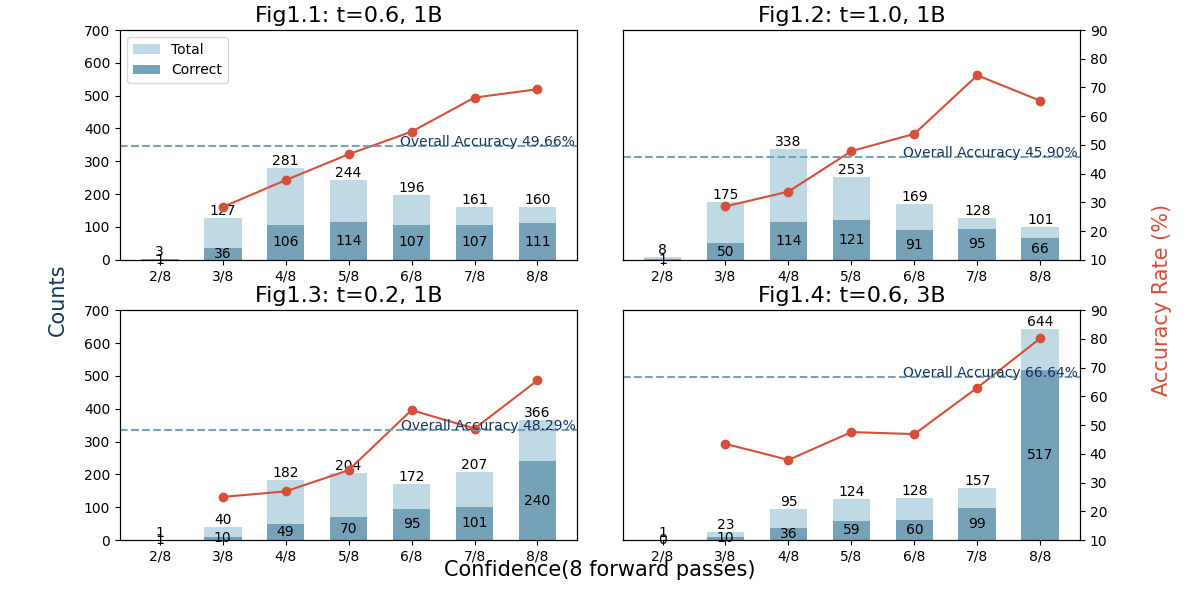
\includegraphics[width=\linewidth]{plot_predictions_2x2.png}
	\caption{Counts of each confidence level \& Overall accuracy for different model and temperature settings.}
	\label{fig:2x2plot}
\end{figure*}

\subsection{Temperature}

Temperature is a parameter that scales the logits (raw prediction scores) before they are transformed into probabilities via the softmax function. A higher temperature results in a more uniform distribution of probabilities, which can lead to more diverse and creative responses from the model. However, this can also increase the likelihood of generating incorrect or nonsensical outputs.

According to Meta's thesis on Llama-3.2\autocite{dubey2024llama3herdmodels}, they explored randomly choosing the temperature hyperparameter from the range of 0.2 to 1 for diverse generations in the early rounds of post-training. With a high temperature, responses can become creative and inspiring but are also more susceptible to unnecessary or unnatural code-switching. As a result, they used a constant value of 0.6 to balance this trade-off in the final round of post-training.

Therefore, we will also examine the temperature hyperparameter within the range of 0.2 to 1. Additionally, we will set a constant value of 0.6 in the following two subsections to check the influence of other settings.

\subsection{Model Scale}

In consideration of simplicity and memory constraint, we here use the two smallest model in the Llama-3.2 family, which are the 1B and 3B parameters model to conduct the experiment. The 1B model has 1.23 billion parameters, while the 3B model has 3.21 billion parameters.\autocite{huggingfaceLlama-3.2-1B-Instruct}

\subsection{Multiple forward passes}

Majority voting can enhance the robustness and accuracy of predictions. The core concept involves combining the outputs from multiple forward passes of the model and selecting the most common output as the final prediction. In this experiment, we begin with 8 forward passes and then evaluate the impact of varying the number of forward passes on the model's accuracy by both doubling and halving the initial number.

%------------------------------------------------

\section{Conclusion}

From Figure \ref{fig:2x2plot}, in each case, at a level of 8 forward passes, the model's accuracy is higher with higher confidence levels. This aligns with the general understanding that more stable responses are more likely to be correct in a normal setting.

\subsection{Temperature}

From Figure \ref{fig:2x2plot}, we can observe that as the temperature increases, the confidence in the model's outputs decreases. This is because a higher temperature results in a flatter probability distribution, leading to more diverse and creative responses. However, this increased diversity can also increase the likelihood of generating incorrect or nonsensical outputs, thereby reducing the overall accuracy of the model. Specifically, the accuracy drops from 49.66\% at a temperature setting of 0.6 to 45.90\% at a temperature setting of 1.0.

\subsection{Model Scale}

The accuracy of the 3B model is significantly higher than that of all 1B models across different settings, with a 66.64\% accuracy compared to the highest 1B model's 51.11\%. Additionally, the overall confidence level is much higher, indicating that the output distribution of the 3B model is more focused and coherent, while also achieving better accuracy. This result aligns with the general understanding that larger models tend to perform better than smaller ones, as they have more parameters and can capture more complex patterns in the data.

\subsection{Multiple forward passes}

\begin{table} % Single column table
	\centering
	\begin{tabular}{l c}
		\toprule
		\multicolumn{2}{l}{Llama-3.2 1B model} \\
		\cmidrule(r){1-1}
		Num of forward passes  & Accuracy \\
		\midrule
		4 &  48.12\% \\
		8 &  49.66\% \\
		16 &  51.11\% \\
		\bottomrule
	\end{tabular}
	\caption{Overall Accuracy(with t = 0.6)}
	\label{tab:accuracy}
\end{table}

From Table \ref{tab:accuracy}, we can see that the accuracy of the model increases as the number of forward passes increases. This is because majority voting helps to reduce the impact of random noise in the model's predictions, leading to more stable and accurate outputs. Specifically, the accuracy increases from 48.12\% with 4 forward passes to 51.11\% with 16 forward passes.

%----------------------------------------------------------------------------------------
%	 REFERENCES
%----------------------------------------------------------------------------------------

\printbibliography % Output the bibliography

%----------------------------------------------------------------------------------------

\end{document}
